%!TEX root =  cpt-rl-icml.tex
We consider a traffic signal control application where the aim is to improve the road user experience by an adaptive traffic light control (TLC) algorithm.
We apply the CPT-functional to the delay experienced by road users, since CPT realistically captures the attitude of the road users towards delays. We then optimize the CPT-value of the delay and contrast this approach with traditional expected delay optimizing algorithms. It is assumed that the CPT functional's parameters $(u,w)$ are given (usually, these are obtained by observing human behavior). The experiments are performed using the GLD traffic simulator \cite{GLDSim}, and the implementation is available at \url{https://bitbucket.org/prashla/rl-gld}.

% \subsection{Simulation Setup}  
We consider a road network with $\N$ signalled lanes that are spread across junctions and $\M$ paths, where each path connects (uniquely) two edge nodes, from which the traffic is generated -- See \cref{fig:2x2grid}. 
%\todoc{Can we have a higher quality figure?}
At any instant $n$, let $q_n^i$ and $t_n^i$ denote the queue length and elapsed time since the lane turned red, for any lane $i = 1,\ldots, \N$. Let $d_n^{i,j}$ denote the delay experienced by $j$th road user on $i$th path, for any $i=1,\ldots,\M$ and $j=1,\ldots,n_i$, where $n_i$ denotes the number of road users on path $i$.
We specify the various components of the traffic control MDP below.
The state $s_n=(q_n^1,\ldots,q_n^{\N},t_n^1,\ldots,t_n^{\N},d_n^{1,1},\ldots,d_n^{\M,n_{\M}})\tr$ is a vector of lane-wise queue lengths, elapsed times and pathwise delays.
The actions are the feasible traffic signal configurations. 

\pgfplotsset{every x tick label/.append style={font=\scriptsize}}

 \begin{figure}
    \centering
     \begin{tabular}{c}
\subfigure[Snapshot of a 2x2-grid network from GLD simulator. The figure shows eight edge nodes that generate traffic, four traffic lights and  four-laned roads carrying cars. ]{
\label{fig:2x2grid}
        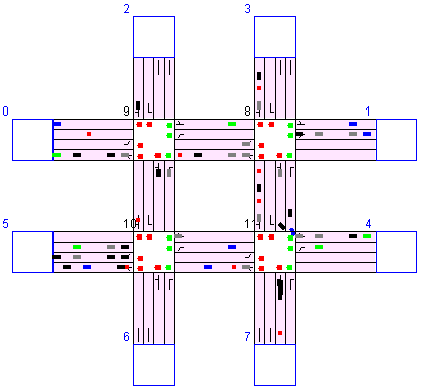
\includegraphics[width=2.3in,height=2in]{fig/2x2grid.png}
}
\\		
\subfigure[AVG-SPSA]{
\label{fig:avg}
\hspace{-2em} 
\tabl{c}{\scalebox{0.75}{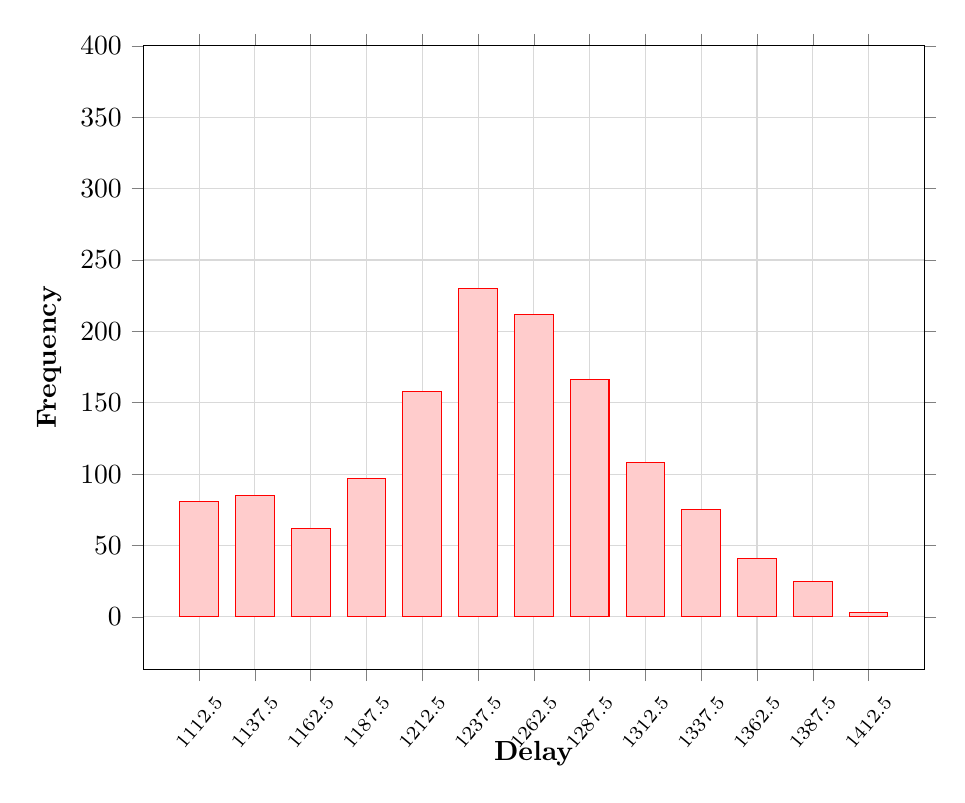
\begin{tikzpicture}
\begin{axis}[
ybar,
ymax=400,
%  legend style={at={(0.5,-0.2)},anchor=north,legend columns=-1},
legend pos=outer north east,
legend image code/.code={\path[fill=white,white] (-2mm,-2mm) rectangle
(-3mm,2mm); \path[fill=white,white] (-2mm,-2mm) rectangle (2mm,-3mm); \draw
(-2mm,-2mm) rectangle (2mm,2mm);},
ylabel={\bf Frequency},
xlabel={\textbf{Delay}},
x label style={at={(axis description cs:0.5,-0.1)},anchor=north},
symbolic x coords={0, 1112.5,1137.5,1162.5,1187.5,1212.5,1237.5,1262.5,1287.5,1312.5,1337.5,1362.5,1387.5,1412.5, 14},
xmin={0},
xmax={14},
xtick=data,
ytick align=outside,
xticklabel style={rotate=50, align=center},
bar width=14pt,
%  bar shift=0pt,
%  enlarge x limits={abs=0.5},
% nodes near coords,
grid,
grid style={gray!30},
width=11.5cm,
height=9.5cm,
]
\addplot[red, fill=red!20]   coordinates { 
(1112.5,81)  (1137.5,85)  (1162.5,62)  (1187.5,97)  (1212.5,158)  (1237.5,230)  (1262.5,212)  (1287.5,166)  (1312.5,108)  (1337.5,75)  (1362.5,41)  (1387.5,25)  (1412.5,3)   };
% 10 breaks: (1125,166) (1175,159) (1225,388) (1275,378) (1325,183) (1375,66) (1425,3)};
% (1000,12) (1050,7) (1100,10)   (1150,35) (1200,137) (1250,248) (1300,375) (1350,324) (1400,138) (1450,19) (1500,10) (1550,1) (1600,0) }; 
% \addplot[darkgreen, fill=darkgreen!20]   coordinates {  (1000,5) (1050,10) (1100,4) (1150,19) (1200,105) (1250,232) (1300,326) (1350,363) (1400,180) (1450,19) (1500,0) (1550,0) (1600,0) }; 
\end{axis}
\end{tikzpicture}}\\[0.5ex]}
}
\\
%%%%%%%%%%%%%%%%%%%%%%%%%
\subfigure[CPT-SPSA]{
\label{fig:cpt}
\hspace{-2em} 
\tabl{c}{\scalebox{0.75}{\begin{tikzpicture}
\begin{axis}[
ybar={2pt},
%  legend style={at={(0.5,-0.2)},anchor=north,legend columns=-1},
ymax=400,
legend pos=outer north east,
legend image code/.code={\path[fill=white,white] (-2mm,-2mm) rectangle
(-3mm,2mm); \path[fill=white,white] (-2mm,-2mm) rectangle (2mm,-3mm); \draw
(-2mm,-2mm) rectangle (2mm,2mm);},
ylabel={\bf Frequency},
xlabel={\textbf{Delay}},
x label style={at={(axis description cs:0.5,-0.1)},anchor=north},
symbolic x coords={0, 1112.5,1137.5,1162.5,1187.5,1212.5,1237.5,1262.5,1287.5,1312.5,1337.5,1362.5,1387.5,1412.5, 14},
xmin={0},
xmax={14},
xtick=data,
ytick align=outside,
xticklabel style={rotate=50, align=center},
bar width=14pt,
% nodes near coords,
grid,
grid style={gray!30},
width=11.5cm,
height=9.5cm,
]
% \addplot[darkgreen, fill=darkgreen!20]   coordinates {  (1100,16) (1150,38) (1200,69) (1250,44) (1300,51) (1350,16) (1400,22) (1450,17) (1500,24) }; 
\addplot[darkgreen, fill=darkgreen!20]   coordinates {  
% (1000,5) (1050,10) (1100,4) (1150,19) (1200,105) (1250,232) (1300,326) (1350,363) (1400,180) (1450,19) (1500,0) 
% 10 breaks: (1110,173)  (1130,176)  (1150,158)  (1170,87)  (1190,33)  (1210,29)  (1230,9)  (1250,1)  
(1112.5,228)  (1137.5,211)  (1162.5,135)  (1187.5,53)  (1212.5,33)  (1237.5,5)  (1262.5,2)  (1287.5,0)  (1312.5,0)  (1337.5,0)  (1362.5,0)  (1387.5,0)  (1412.5,0)  
}; 
 

\end{axis}
\end{tikzpicture}}\\[0.5ex]}
}
\end{tabular}
\caption{Histogram of the sample delays for the path from node $0$ to $4$ (see Figure \ref{fig:2x2grid}) for AVG-SPSA that minimizes overall expected  delay (see \eqref{eq:avg-traffic}) and CPT-SPSA that maximizes CPT-value of differential delay (see \eqref{eq:cpt-traffic}. }
\label{fig:histogram-perf}
\end{figure}

We consider Boltzmann policies that have the form
$$
\pi_{\theta}(s,a) = \frac{e^{\theta^{\top} \phi_{s,a}}}{\sum_{a' \in {\A(s)}} e^{\theta^{\top} \phi_{s,a'}}},
\hspace{6pt} \forall s \in \S,\;\forall a \in \A(s),
$$
with features $\phi_{s,a}$ as described in Section V-B of \cite{prashanth2012threshold}.
% We consider two different notions of return as follows:
% %
% \textbf{CPT:} 
For any policy $\theta$, let $X_i^\theta$ be the delay r.v. and $\mu_i^\theta$ the proportion of road users along path $i$, for $i=1,\ldots,\M$. 
Any road user along path $i$ will evaluate the delay (s)he experiences in a manner that is captured well by CPT. 
An important component of CPT is to employ a reference point to calculate gains and losses. 
%Choosing a suitable reference point is challenging, but \cite{tversky1992advances} advocate using status-quo as the reference point. 
In our setting, we use path-wise delays, say $B_i$ for path $i$, obtained from a pre-timed TLC (cf. the Fixed TLCs in \cite{prashanth2011reinforcement}) as the reference point.
If the delay of any TLC algorithm is less than that of pre-timed TLC, then the (positive) difference in delays is perceived as a gain and in the complementary case, the delay difference is perceived as a loss. Thus, the CPT-value $\C(B_i-X_i)$ for any path $i$ in \eqref{eq:cpt-traffic} is to be understood as a \textit{differential delay} w.r.t. $B_i$.  
Now, the objective is to maximize the weighted sum of CPT-values across paths, i.e., 
% With the objective of maximizing the experience of road users across paths, the overall return to be optimized is given by
\begin{align}
\max_{\theta \in \Theta} \text{CPT}(X_1^\theta,\ldots,X_{\M}^\theta) = \sum_{i=1}^{\M} \mu_i^\theta \C(B_i - X_i^\theta),\label{eq:cpt-traffic}
\end{align}
where $\Theta$ is the $d$-dimensional hypercube formed by intervals $[0.1,1.0]$ in each dimension.  
% where  $\C(B_i-X_i)$ is the CPT-value along path $i$ for differential delay r.v. $B_i-X_i$. 
% \textbf{EUT:} Here we only use the utility functions $u^+$ and $u^-$ to handle gains and losses, but do not distort probabilities. 
% Thus, the EUT objective is defined as
% \begin{align*}
% \text{EUT}(X_1,\ldots,X_{\M}) = \sum_{i=1}^{\M} \mu^i \left(\E(u^+(X_i) - \E(u^-(X_i)\right),
% \end{align*}
% where $\E(u^+(X_i)) = \intinfinity \Prob{u^+(X_i)>z} dz$ and $\E(u^-(X_i)) - \intinfinity \Prob{u^-(X_i)>z} dz$, for $i=1,\ldots,\M$.

For the sake of comparison, we consider the traditional objective of minimizing the overall average delay, i.e.,
\begin{align}
\min_{\theta\in \Theta}\text{AVG}(X_1^\theta,\ldots,X_{\M}^\theta) = \sum_{i=1}^{\M} \mu_i^\theta \E(X_i^\theta). \label{eq:avg-traffic} 
\end{align}
In comprison to CPT objective, the above does not incorporate baseline delays, makes no distinction between gains and losses via utility functions and does not distort probabilities. 
%Thus, the AVG objective is defined as
%\begin{align}
%\text{AVG}(X_1,\ldots,X_{\M}) = \sum_{i=1}^{\M} \mu^i \E(X_i).
%\end{align}   
%where $\E(X_i) = \intinfinity P(u^+(X_i)>z) dz - \intinfinity P(u^-(X_i)>z) dz$.
% An important component of CPT is to employ a reference point to calculate gains and losses. 
% %Choosing a suitable reference point is challenging, but \cite{tversky1992advances} advocate using status-quo as the reference point. 
% In our setting, we use path-wise delays obtained from a pre-timed TLC (cf. the Fixed TLCs in \cite{prashanth2011reinforcement}) as the reference point. If the delay of any TLC algorithm is less than that of pre-timed TLC, then the (positive) difference in delays is perceived as a gain and in the complementary case, the delay difference is perceived as a loss. Thus, the CPT-value $\C(X_i)$ for any path $i$ in \eqref{eq:cpt-traffic} is to be understood as a \textit{differential delay}.  
% 
% %, as the road network considered is high-dimensional (state space cardinality $> 10^{60}$). 
% 
% Using a Boltzmann policy that has the form
% $$
% \pi_{\theta}(s,a) = \frac{e^{\theta^{\top} \phi_{s,a}}}{\sum_{a' \in {\A(s)}} e^{\theta^{\top} \phi_{s,a'}}},
% \hspace{6pt} \forall s \in \S,\;\forall a \in \A(s),
% $$
% with features $\phi_{s,a}$ as described in Section V-B of \cite{prashanth2012threshold},
% 

We implement the following TLC algorithms:

{\bf\em CPT-SPSA}: This is a first-order algorithm (see Algorithm \ref{alg:1spsa}) that solves \eqref{eq:cpt-traffic} using SPSA-based gradient estimates and the scheme from Algorithm \ref{alg:holder-est} for estimating CPT-value \\$\C(B_i-X_i)$ for each path $i=1,\ldots,\M$, with $d_n^{i,j}, j=1,\ldots,n_i$ as the samples.

% {\bf\em EUT-SPSA}: This is similar to CPT-SPSA, except that weight functions $w^+(p)=w^-(p)=p,$ for $p\in [0,1]$. 

{\bf\em AVG-SPSA}: This is SPSA-based first-order algorithm that solves \eqref{eq:avg-traffic}, while using sample averages of the delays to estimate the expected delay $\E(X_i)$ for each path $i=1,\ldots,\M$. 

As in Section \ref{sec:expts-simple}, the utility functions underlying the CPT-value $\C(X_i), \forall i$ have the form
$$u^+(x) =  |x|^{\sigma} \text{ and  }u^-(x) = \lambda |x|^{\sigma},$$ 
where $\lambda = 2.25$ and $\sigma = 0.88$.
The weight functions $w^+,w^-$ are set as follows:
\begin{align*}
w^+(p) &= \frac{p^{\eta_1}}{{(p^{\eta_1}+ (1-p)^{\eta_1})}^{\frac{1}{\eta_1}}}, w^-(p) = \frac{p^{\eta_2}}{{(p^{\eta_2}+ (1-p)^{\eta_2})}^{\frac{1}{\eta_2}}},
\end{align*} 
where $\eta_1 = 0.61$ and $\eta_2 = 0.69$. The choices for $\lambda$, $\sigma$, $\eta_1$ and $\eta_2$ are based on median estimates given by \cite{tversky1992advances} and have been used earlier in a traffic application (see \cite{gao2010adaptive}).
For all the algorithms,
 motivated by standard guidelines (see \cite{spall2005introduction}),
 we set $\delta_n = 1.9/n^{0.101}$ and $a_n = 1/(n+50)$. The initial point $\theta_0$ is the $d$-dimensional vector of ones and $\forall i$, the operator $\Gamma_i$ keeps the iterate $\theta_i$ bounded within $[0.1, 1.0]$.

\begin{table}
 \centering
  \caption{AVG and CPT-value estimates for AVG-SPSA and CPT-SPSA algorithms. Note: CPT-value is of differential delays w.r.t. pre-timed TLC, while 
  AVG-value uses absolute delays.}
  \label{tab:cpt-results}
 \begin{tabular}{|c|c|c|}
  \toprule 
   & \textbf{AVG-value}& \textbf{CPT-value }\\\midrule
   AVG-SPSA & $\bm{1596.55}$ & $624.68$ \\\midrule
   CPT-SPSA & $1744.94$ & $\bm{659.61}$\\
   \bottomrule
  \end{tabular}
%   
%   \vspace{1ex}
%   
\end{table}

 
The experiments involve two phases:
first, a training phase where we run each algorithm for $1000$ iterations, with each iteration involving two perturbed simulations. Each simulation involves running the traffic simulator with a fixed policy parameter for $2000$ steps and this corresponds to approximately $2000$ delay samples. The training phase is followed by a test phase where we fix the policy obtained at the end of training (i.e., after $1000$ iterations of SPSA) and then run the traffic simulator with the aforementioned parameter for $30000$ steps. 

% \subsection{Results} 

Figures \ref{fig:avg}--\ref{fig:cpt} present the histogram of the delays for the path from node $0$ to node $4$, obtained from the test phase for AVG-SPSA and CPT-SPSA, respectively.  
% A similar exercise for pre-timed TLC resulted in a CPT-value of $-46.14$. 
It is evident that each algorithm converges to a different policy and the difference, in $\ell_1$ norm, between policy parameters obtained at the end of training phase for AVG-SPSA and CPT-SPSA was observed to be $6.51$. 
% As shown in Table \ref{tab:cpt-results},  AVG-SPSA results in a TLC policy with lower expected delay, while CPT-SPSA's policy has higher CPT-value. This is expected because AVG-SPSA uses neither utilities nor probability distortions and minimizes overall delay, while CPT-SPSA uses a pre-timed TLC baseline and treats delay gains and losses differently. 
Interestingly, from Figures \ref{fig:avg}--\ref{fig:cpt} we observe that CPT-SPSA results in a left-skewed delay distribution that avoids higher delay values, while the delay distribution of AVG-SPSA is closer to a bell-shape. While the histograms are for a single path $0-4$, we observed similar trends in the paths originating at node $0$ and node $7$, which constitute the bulk of the traffic volume. As shown in Table \ref{tab:cpt-results}, AVG-SPSA is better than CPT-SPSA in terms of expected delay, but CPT-SPSA results in a higher CPT value.

The results in this as well as in the previous section argue for specialized algorithms for optimizing CPT-based criteria, since expected value optimizing algorithms cannot be used as surrogates. 
% esp. in the light of previous findings which show CPT matches human evaluation well and there is a need for algorithms that serve human needs well.
%\todoc{It would be nice to point out how the CPT policy is different than the others.}

